\documentclass{article}
\usepackage{amsmath}
\usepackage{mathtext}
\usepackage[T1,T2a]{fontenc}
\usepackage[utf8]{inputenc}
\usepackage[english, bulgarian, russian]{babel}
\usepackage{tikz}
\usepackage{pgfplots}
\usepackage[export]{adjustbox}
\usepackage[left=2cm,right=2cm,
    top=2cm,bottom=2cm,bindingoffset=0cm]{geometry}

\title{Определение моментов инерции твердых тел с помощью трифилярного подвеса}
\date{2019-11-11}
\author{Панферов Андрей}

\begin{document}
\topmargin=-10mm
\pagenumbering{gooble}
\maketitle
\newpage
\pagenumbering{arabic}

\section{Аннотация}
В работе проверяются теоретические расчеты моментов инерции некоторых тел и проверка теоремы Гюйгенса-Штейнера с помощью трифилярного подвеса. \\ полить воды
\section{Теоретические сведения}

Платформа Р укреплена на кронштейне и снабжена рычагом, при помощи которого в системе можно создать крутильные колебания путем небольшого поворота верхней платформы. 
После того, как нижняя платформа Р' оказывается повернутой на угол &{\phi}& относительно верхней платформы Р, возникает момент сил, стремящийся вернуть нижнюю платформу в положение равновесия, при котором относительный поворот платформ отсутсвует. Но в положении равновесия платформа не останавливается, так как имеет угловую скорость. В результате платформа совершает крутильные колебания.
Если пренебречь потерями энергии на трение, то уравнение сохранения энергии при колебаниях можно записать таким образом: 

\begin{align*}
   \frac{I\dot \phi^2}{2} + mg(z_0-z) &= E\\
\end{align*}

Расстояние между точками С и С'' равно длине нити L.

\begin{align*}
   (Rcos\phi - r)^2\+R^2sin^2\phi+z^2 &= L^2\
\end{align*}

Учитывая малость угла поворота и пользуясь первым приближением корня получим:

\begin{align*}
   z &\approx z_0-\frac{Rr\phi^2}{2z_0}\
\end{align*}

Подставляем это выражение в закон сохранения энергии, дифференцируем уравнение сохранения по времени и сокращаем на &{\dot \phi}&. Находим уравнение крутильных колебаний:

\begin{align*}
   I \ddot {\phi} + mg\frac{Rr}{z_0}\phi&=0\\
\end{align*}

Откуда

\begin{align*}
   T&=2\pi\sqrt{\frac{Iz_0}{mgRr}} & I = \frac{mgRrT^2}{4\pi^2z_0} && k = \frac{grR}{4\pi^2z_0} &&& I=kmT^2\\
\end{align*}

\section{Оборудование и инструментальные погрешности}
Трифилярный подвес, секундомер, счетчик числа колебаний, набор тел, момент инерции которых надлежит измерить -- используются в качестве оборудования.
Формулы для расчета погрешностей:

\begin{align*}
  \frac{\Delta z_0}{z_0} &= \sqrt{4(\frac{\Delta R}{R})^2+4(\frac{\Delta r}{r})^2+4(\frac{\Delta h}{h})^2} \\
   \frac{\Delta k}{k} &= \sqrt{5(\frac{\Delta R}{R})^2+5(\frac{\Delta r}{r})^2+4(\frac{\Delta h}{h})^2}\\
   \frac{\Delta I_i}{I_i} &= \sqrt{(\frac{\Delta k}{k})^2+4(\frac{\Delta T}{T})^2+(\frac{\Delta m_i}{m_i})^2}\\
   \frac{\Delta m}{m} &= \sqrt{4(\frac{\Delta k}{k})^2+4(\frac{\Delta \lambda}{\lambda})^2+(\frac{\Delta m_0}{m_0})^2}\\
\end{align*}
\begin{align*}
   \frac{\Delta I_{диска}}{I_{диска}} &= \sqrt{4(\frac{\Delta k}{k})^2+4(\frac{\Delta \lambda}{\lambda})^2+(\frac{\Delta m_0}{m_0})^2+(\frac{\Delta \sigma}{\sigma})^2+(\frac{\Delta I_0}{I_0})^2}
\end{align*}

\section{Измерение параметров установки}

\begin{minipage}[h]{0.30\linewidth}
	\centering
	\caption{Параметры установки:}
	\begin{align*}
	z_0 =& \: 2.146 \pm 0.02 м& \\
	R =& \: 114.6 \pm 0.5 мм& \\
	r =& \: 30.5 \pm 0.3 мм& \\
	k =& \: \frac{grR}{4 \pi^2 \cdot z_0} = \: (4.03 \pm 0.06)\cdot 10^{-4} м^2/с^2 \\
	m =& \: 983.2 \pm 0.5 г
	\end{align*}
\end{minipage}
\begin{minipage}[h]{0.60\textwidth}
	\centering
	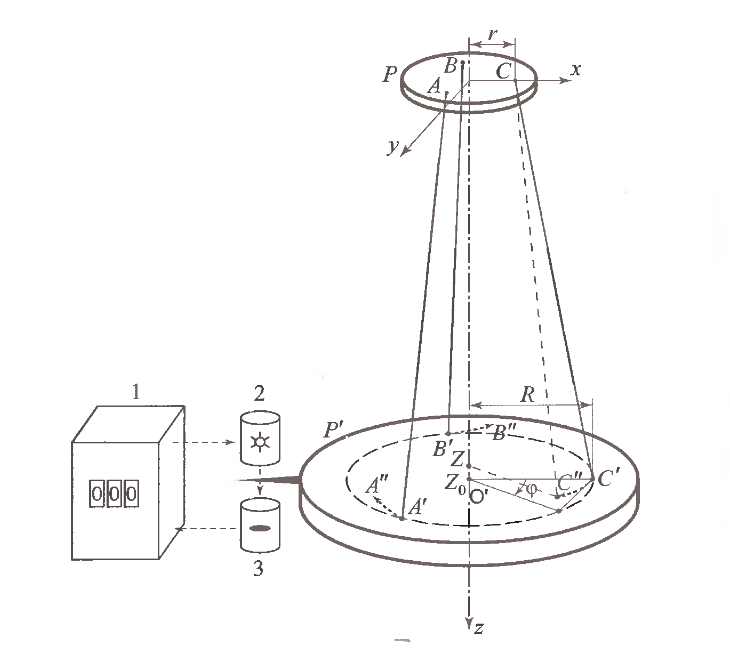
\includegraphics[width=1\linewidth]{Podves.png}
\end{minipage}

\section{Колебания пустой платформы}

	\begin{table}[h!]
	\begin{center}
	\caption{Серия измерения периодов}
	\begin{tabular}{|c|c|c|c|c|c|c|c||c|c|}
		\hline
		$T_{10}$, с&43.942&43.886&43.885&43.872&43.886&43.874&43.884&$T_{10ср} = 4.3890c$&$\delta T_{10ср} = 0.0009c$\\
		\hline
	\end{tabular}
	\end{center}
	\end{table}
	\begin{equation*}
	I_{0} =& \: (7.63 \pm 0.11) \cdot 10^{-3} кг \cdot м^2
	\end{equation*}
\section{Измерение моментов инерции тел}

	\subsection{Диск}
	
	\begin{equation*}
	m = \: 584.4 г \ \ \ ; \ \ r = 85.4 мм 
	\end{equation*}

	\begin{table}[h!]
	\begin{center}
	\begin{tabular}{|c|c|c|c|c|c|c|c||c|c|}
		\hline
		$T_{10}$, с&39.292&39.292&39.277&39.225&39.286&39.238&39.212&$T_{10ср} = 3.9260c$&$\delta T_{10ср} = 0.0013c$\\
		\hline
	\end{tabular}
	\end{center}
	\end{table}
	\begin{equation*}
	I_{диск} =& \: (2.11 \pm 0.20) \cdot 10^{-3} кг \cdot м^2
	\end{equation*}

\newpage

	\subsection{Брусок}

	\begin{equation*}
	m = \: 1273.0 г \ \ \ ; \ \ l = 209.2 мм \ \ \ ; \ \ b = 28.5 мм 
	\end{equation*}

	\begin{table}[h!]
	\begin{center}
	\begin{tabular}{|c|c|c|c|c|c|c|c||c|c|}
		\hline
		$T_{10}$, с&36.998&36.975&36.926&36.971&36.994&36.919&36.958&$T_{10ср} = 3.6963c$&$\delta T_{10ср} = 0.0012c$\\
		\hline
	\end{tabular}
	\end{center}
	\end{table}
	\begin{equation*}
	I_{брусок} =& \: (4.79 \pm 0.22) \cdot 10^{-3} кг \cdot м^2
	\end{equation*}

	\subsection{Кольцо}

	\begin{equation*}
	m = \: 776.9 г \ \ \ ; \ \ r = 154.3 мм 
	\end{equation*}

	\begin{table}[h!]
	\begin{center}
	\begin{tabular}{|c|c|c|c|c|c|c|c||c|c|}
		\hline
		$T_{10}$, с&41.747&41.718&41.720&41.707&41.701&41.695&41.689&$T_{10ср} = 4.1611c$&$\delta T_{10ср} = 0.0008c$\\
		\hline
	\end{tabular}
	\end{center}
	\end{table}
	\begin{equation*}
	I_{диск} =& \: (4.65 \pm 0.13) \cdot 10^{-3} кг \cdot м^2
	\end{equation*}

	\subsection{Кольцо+Диск}

	\begin{equation*}
	m = \: 1361.3 г
	\end{equation*}

	\begin{table}[h!]
	\begin{center}
	\begin{tabular}{|c|c|c|c|c|c|c|c||c|c|}
		\hline
		$T_{10}$, с&39.112&39.121&39.120&39.059&39.045&39.105&39.103&$T_{10ср} = 3.9095c$&$\delta T_{10ср} = 0.0009c$\\
		\hline
	\end{tabular}
	\end{center}
	\end{table}
	\begin{equation*}
	I_{диск} =& \: (6.81 \pm 0.15) \cdot 10^{-3} кг \cdot м^2
	\end{equation*}

	\subsection{Кольцо+Диск+Брусок}

	\begin{equation*}
	m = \: 2634.3 г
	\end{equation*}

	\begin{table}[h!]
	\begin{center}
	\begin{tabular}{|c|c|c|c|c|c|c|c||c|c|}
		\hline
		$T_{10}$, с&36.343&36.292&36.285&36.272&36.347&36.360&36.350&$T_{10ср} = 3.6321c$&$\delta T_{10ср} = 0.0014c$\\
		\hline
	\end{tabular}
	\end{center}
	\end{table}
	\begin{equation*}
	I_{диск} =& \: (11.60 \pm 0.21) \cdot 10^{-3} кг \cdot м^2
	\end{equation*}

	\subsection{Сравнение теории с результатами эксперимента}

	\begin{tabular}{|c|c|c|c|c|c|}
	\hline
	Образец&Диск&Брусок&Кольцо&Диск+Кольцо&Диск+Кольцо+Брусок\\
	\hline
	$I_{эксп}$, $кг \cdot м^2 \cdot 10^{-3}$&$2.11 \pm 0.20$&$4.79 \pm 0.22$&$4.65 \pm 0.13$&$6.81 \pm 0.15$&$11.60 \pm 0.21$\\
	\hline
	$I_{теор}$, $кг \cdot м^2 \cdot 10^{-3}$&2.13&4.73&4.62&6.75&11.48\\
	\hline
	\end{tabular}

\newpage

\section{Проверка закона Гюгенса-Штейнера}

\begin{equation*}
\end{equation*}

\begin{left}
Параметры образца:
\begin{equation*}
\left
r = 90.0 мм \ \ \ ; \ \ \delta x = 5 мм \\
\
\end{equation*}

\begin{equation*}
\end{equation*}

\end{left}
\begin{minipage}[h]{0.30\textwidth}
	\centering
	\begin{tabular}{|c|c|}
	\hline
	n&$T_{10}$, c\\
	\hline
	0&30.799\\
	\hline
	1&30.830\\
	\hline
	2&30.923\\
	\hline
	3&31.267\\
	\hline
	4&31.722\\
	\hline
	5&32.233\\
	\hline
	6&32.871\\
	\hline
	7&33.536\\
	\hline
	8&34.388\\
	\hline
	9&35.308\\
	\hline
	10&36.134\\
	\hline
	\end{tabular}
\end{minipage}
\begin{minipage}[h]{0.69\textwidth}

\begin{tikzpicture}[scale = 1]
\begin{axis}[
    axis lines = left,
    legend style={at={(0.9, 0.3)}},
    xlabel = {$n^2$},
    ylabel = {$T^2$, c},
    xmin=0, xmax=100,
    ymin=9, ymax=14,
	ymajorgrids = true,
	xmajorgrids = true
]
\addplot[
	mark = square, 
	mark options = {
		scale = 1.5, 
		fill = red, 
		draw = chucknorris
	},
	ymajorgrids = true,
	xmajorgrids = true,
	color = blue 
]  coordinates {
	(0, 9.486) (1, 9.504) (4, 9.562) (9, 9.776) (16, 10.063) (25, 10.390) (36, 10.805) (49, 11.247) (64,11.825) (81,12.467) (100,13.056)};

\addplot [
    domain=0:100, 
    samples=1000, 
    color=red,
]
{9.399+x*0.03689};


\legend{ 
	Эксперимент,
	Теория
};

\end{axis}
\end{tikzpicture}

\end{minipage}

\section{Обсуждение результатов и выводы}
Мы выяснили, что теоретические выводы моментов инерции верны и совпадают с экспериментальными данными. Так же мы выяснили, что момент инерции аддитивен, а закон Гюйгенса-Штейнера выполняется, так как линеаризованная зависимость получилась прямой.
Погрешности величин не превышают 10\%

\end{document}